% vim: set tw=0:
\documentclass{beamer}
\usepackage{graphicx}
\usepackage{hyperref}
\hypersetup{pdfborder={0 0 0 0}}

% Reasonable themes:
% Antibes Bergen Berkeley Berlin Frankfurt Goettingen Ilmenau Luebeck Malmoe
% Montpellier PaloAlto Rochester Singapore Szeged Warsaw bars boxes
% compatibility default lined plain shadow sidebar split tree
% And these ones include the author's name on every slide:
% Berkeley

% Declare themes.
\mode<presentation>
\usetheme{UWHEP}

% Personal macros.
\newcommand{\email}[1]{{\texttt #1}}
\newcommand{\newframe}[1]{\section{#1}
    \frametitle{\sc{#1}}}
\newcommand{\subframe}[1]{\subsection{#1}
    \frametitle{\sc{#1}}}
\newcommand{\supers}[1]{\ensuremath{^\textrm{#1}}}
\newcommand{\subs}[1]{\ensuremath{_\textrm{#1}}}
\newcommand{\ca}{\ensuremath{\sim}}
\renewcommand{\email}[1]{\href{mailto:#1}{\nolinkurl{#1}}}

% Author information.
\title{Storage at UW-Madison CMS Tier-2}
\author[Maier]{
    Will Maier \\ 
    {\tt wcmaier@hep.wisc.edu}}
\institute[Wisconsin]{University of Wisconsin - High Energy Physics}
\date[2009.06.30]{OSG Storage Forum, FNAL}
\logo{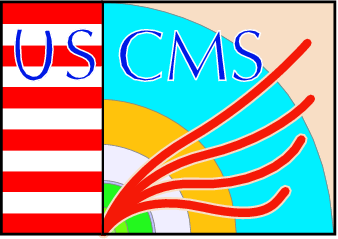
\includegraphics[height=0.6cm]{../../../Graphics/USCMS_logo.png}\hspace{.1cm}
\includegraphics[height=0.75cm]{../../../Graphics/UW_logo.png}}

\begin{document}

% http://indico.fnal.gov/conferenceOtherViews.py?view=standard&confId=2538
% 20 min
% Type of storage    
% Hardware
% Software configuration
% Deployment/ upgrade method
% Usage patterns
% Monitoring, troubleshooting
% Grievances
% Support expectations

\begin{frame}
    \titlepage
\end{frame}

\section{Overview}
\begin{frame}
    \tableofcontents
\end{frame}

\section{Hardware}
\begin{frame}
%\frametitle{}
\begin{itemize}
	\item Emphasize reliability and performance on central servers
	\begin{itemize}
		\item Reliability first: performance means nothing if the systems aren't up\ldots{}
		\item \ldots{}but work doesn't get done if clients are waiting to perform lookups on the central services
	\end{itemize}
	\item Make use of any and all available machines as cluster nodes
	\begin{itemize}
		\item Dedicated servers with large, local filesystems
		\item Batch nodes
		\item Retired test systems
	\end{itemize}
\end{itemize}
\end{frame}

\subsection{Network Topology}
\begin{frame}
\begin{itemize}
	\item 10Gbps fiber uplink to campus, world
	\item XXX network diagram
	\item XXX 10 Cisco 3750Gs bridged to 2 3750Gs over 4Gbps copper Etherchannel
	\item 1Gbps Ethernet to all nodes and central servers
	\item \ca{} XXX TB and XXX nodes on one side; XXX TB and XXX nodes on the other
\end{itemize}
\end{frame}

\subsection{Central Services}
\begin{frame}
\begin{itemize}
	\item Fast RAID for namespace database (up to 200MB/s)
	\begin{itemize}
		\item Need speed: database journals require lots of writes
		\item Need reliability: lots of pain if the database dies or becomes corrupted
		\item At Wisconsin: LSI RAID10 (4x250 GB 10k RPM SATA disks)
	\end{itemize}
	\item Databases and dCache daemons make use of available memory
	\begin{itemize}
		\item At least 2GB/core; most servers have 16GB for 4 cores
	\end{itemize}
	\item Otherwise, commodity hardware
	\begin{itemize}
		\item Fewer configuration profiles to manage
		\item Standard 72000 RPM SATA disks sufficient; no RAID (only namespace needs to persist)
	\end{itemize}
\end{itemize}
\end{frame}

\subsection{Cluster nodes}

\section{Software}

\section{Administration}
\subsection{Deployment}
\subsection{Monitoring}

\section{Experiences}
\subsection{Usage}
\subsection{Support}

\subsection{Plans}
\begin{frame}
\begin{itemize}
	\item Centralize databases on high-performance server or provide faster disks on all central servers
	\item Improve switch port efficiency so all nodes communicate across the same 16Gbps backplane
\end{itemize}
\end{frame}

%\section{}
%\subsection{}
\begin{frame}
%\frametitle{}
\begin{itemize}
	\item ...
\end{itemize}
\end{frame}

\end{document}
